\documentclass[11pt]{article}
\usepackage[utf8]{inputenc}
\usepackage{graphicx}
\graphicspath{ {res/} }
\usepackage{svg}
\usepackage{hyperref}
\usepackage{todonotes}
\usepackage{fontawesome}
\usepackage{pdfpages}
\usepackage[a4paper,width=150mm,top=25mm,bottom=25mm]{geometry}

\title{
\centering
\begin{minipage}{4cm}
    \centering
    \includesvg[width=4cm]{res/ai-center.svg}
\end{minipage}
\hfill % Add horizontal space
\begin{minipage}{4cm}
    \centering
    \includesvg[width=4cm]{res/un.svg}
\end{minipage}\\[1cm] % Add vertical space
{\large Practical Work - Project Report}\\
\textbf{SemUN: A Semantics-Powered Search Platform for the United Nations' Digital Library}
}



\author{
    Clément Sicard\\
    \texttt{csicard@ethz.ch}\\
    D-INFK, ETH Zurich\\
    \\
    \textit{Supervised by:}\\
    Dr. Menna El-Assady$^1$, Dr. Sascha Langenbach$^1$, Catherine Pysden, MSc.$^2$\\
    \\
    $^1$ETH Zurich $^2$United Nations
    }

\begin{document}

\maketitle
\todo[inline]{A faire}

\begin{center}
    \small\textbf{Keywords}:\\
    \textit{
        Natural Language Processing (NLP),
        Named Entity Recognition (NER),
        Graph databases,
        Frontend,
        Network Visualization
    }
\end{center}

\section{Introduction} \label{sec:introduction}
The \href{https://digitallibrary.un.org/}{United Nations Digital Library (UNDL)} is a United Nations (UN) service that provides public access to a diverse range of UN documents: voting data, speeches, maps, and open access publications starting from 1979.
All of these documents have been classified according to the \href{https://metadata.un.org/thesaurus/about?lang=en}{UNBIS Thesaurus}, a multilingual database of the controlled vocabulary used to describe UN documents and other materials in the Library's collection, with a more or less precise topic label.


The main idea of this project is to create an analysis platform, with a network visualization of documents from a subset of the documents in the UN Digital Library. The analytics platform includes a basic Named Entity Recognition (NER) system to extract mentioned entities from the documents. The visualization part will be a network visualization, leveraging the versatility of the structure of a graph to display the extracted insights. Both parts aim at improving the search of documents by implementing an analytics layer on top of the existing search engine from the digital library.

\section{Motivation \& Scope} \label{sec:motivation-scope}

In the short-term, the goal of this project is to provide a MVP of a potential future UN product, in close contact with UN staff to make it conform to their needs. Specifically, this project will focus – as a first iteration – on Catherine Pysden's suggestion, "Women in Peacekeeping".

The project's long-term scope is to be used as a search engine for UN staff, member-state delegates, and members of the general public with an interest in UN topics. Potential future work could include extending the project to the whole UN Digital Library. It could, for instance, also suggest Thesaurus-compliant metadata for untagged documents to facilitate the work of Library staff.


\begin{figure}[!htb]
    \centering
    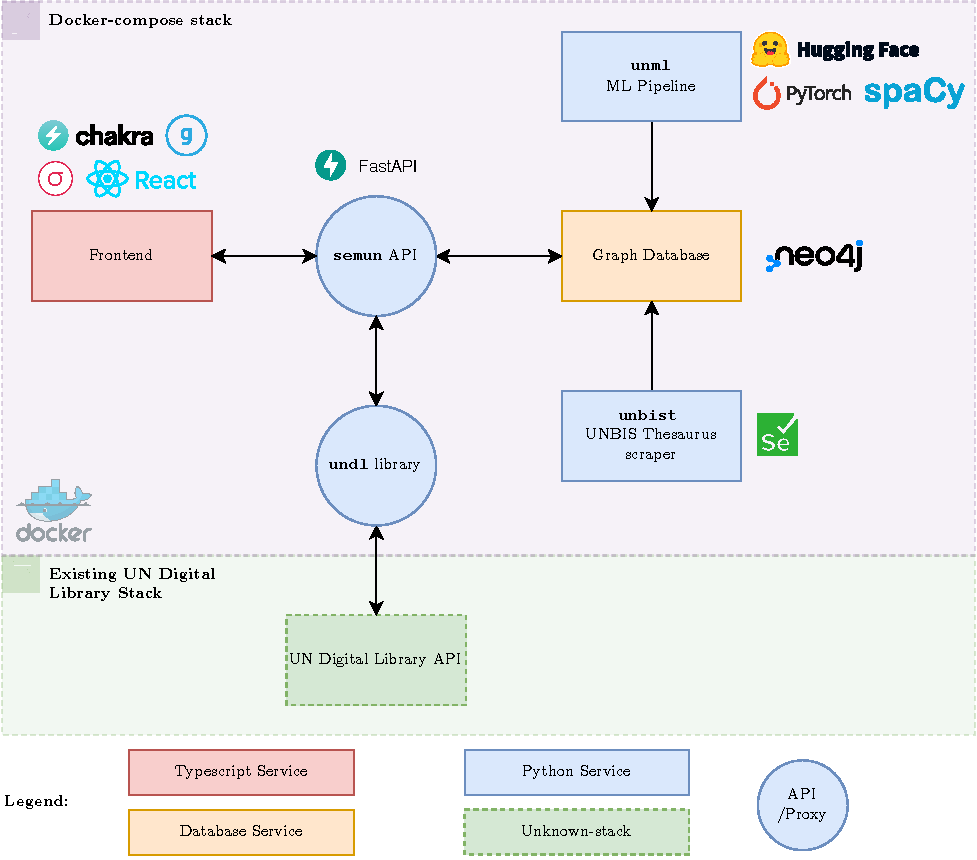
\includegraphics[width=\textwidth]{res/architecture-final.pdf}
    % \includegraphics*[width=0.8\textwidth]{res/architecture-final.png}
    \caption{Final stack architecture}
    % change caption position to the bottom

    \label{fig:architecture}
\end{figure}

\section{Final architecture} \label{sec:final-architecture}

The final architecture is a full-stack architecture, from the database to the frontend, handed in as a Docker compose stack: \href{https://github.com/ClementSicard/un-semun}{\faGithub{} \texttt{un-semun}}.

The project consists of $7$ \faGithub{} Github repos:

\begin{itemize}
    \item \href{https://github.com/ClementSicard/un-semun}{\faGithub{} \texttt{un-semun}}: The main repository with the \texttt{docker-compose} stack declaration.
    \item \href{https://github.com/ClementSicard/un-semun-frontend}{\faGithub{} \texttt{un-semun-frontend}}: The frontend.
    \item \href{https://github.com/ClementSicard/un-semun-api}{\faGithub{} \texttt{un-semun-api}}: The API for the frontend.
    \item \href{https://github.com/ClementSicard/undl}{\faGithub{} \texttt{undl}}: The code for \texttt{undl}, a Python wrapper around the UN Digital Library API.
    \item \href{https://github.com/ClementSicard/un-unbis-thesaurus-scraper}{\faGithub{} \texttt{un-unbis-thesaurus-scraper}}: A scraper for the UNBIS Thesaurus taxonomy website.
    \item \href{https://github.com/ClementSicard/un-ml-pipeline}{\faGithub{} \texttt{un-ml-pipeline}}: Machine learning pipeline for UNDL documents.
    \item \href{https://github.com/ClementSicard/un-semun-misc}{\faGithub{} \texttt{un-semun-misc}}: Diverse scripts used for the project.
    \item \href{https://github.com/ClementSicard/un-semun-paper}{\faGithub{} \texttt{un-semun-paper}}: The code for this paper.
\end{itemize}

This paper will go through each of them in detail except for the paper repository.

\subsection{\texttt{un-semun}: The main repository} \label{ssec:un-semun-the-main-repository}


\subsection{\texttt{un-semun-frontend}: A React \& Sigma.js frontend} \label{ssec:un-semun-frontend-a-react-sigma-js-frontend}
\subsubsection*{Tech stack of \texttt{un-semun-frontend}} \label{sssec:tech-stack-of-un-semun-frontend}

I used React combined with Typescript for the UI framework, as well as \href{https://chakra-ui.com/}{Chakra UI} for the UI components and \href{https://www.sigmajs.org/}{\texttt{Sigma.js}} via its React adapter \href{https://sim51.github.io/react-sigma/}{\texttt{@react-sigma}} for the network map. \href{https://graphology.github.io/}{\texttt{graphology}} was also used for graph manipulation in the frontend, mostly to iterate over graph elements to perform styling. The code is available here: \href{https://github.com/ClementSicard/un-semun-frontend}{\faGithub{} \texttt{un-semun-frontend}}.



\begin{figure}[!htb]
    \centering

    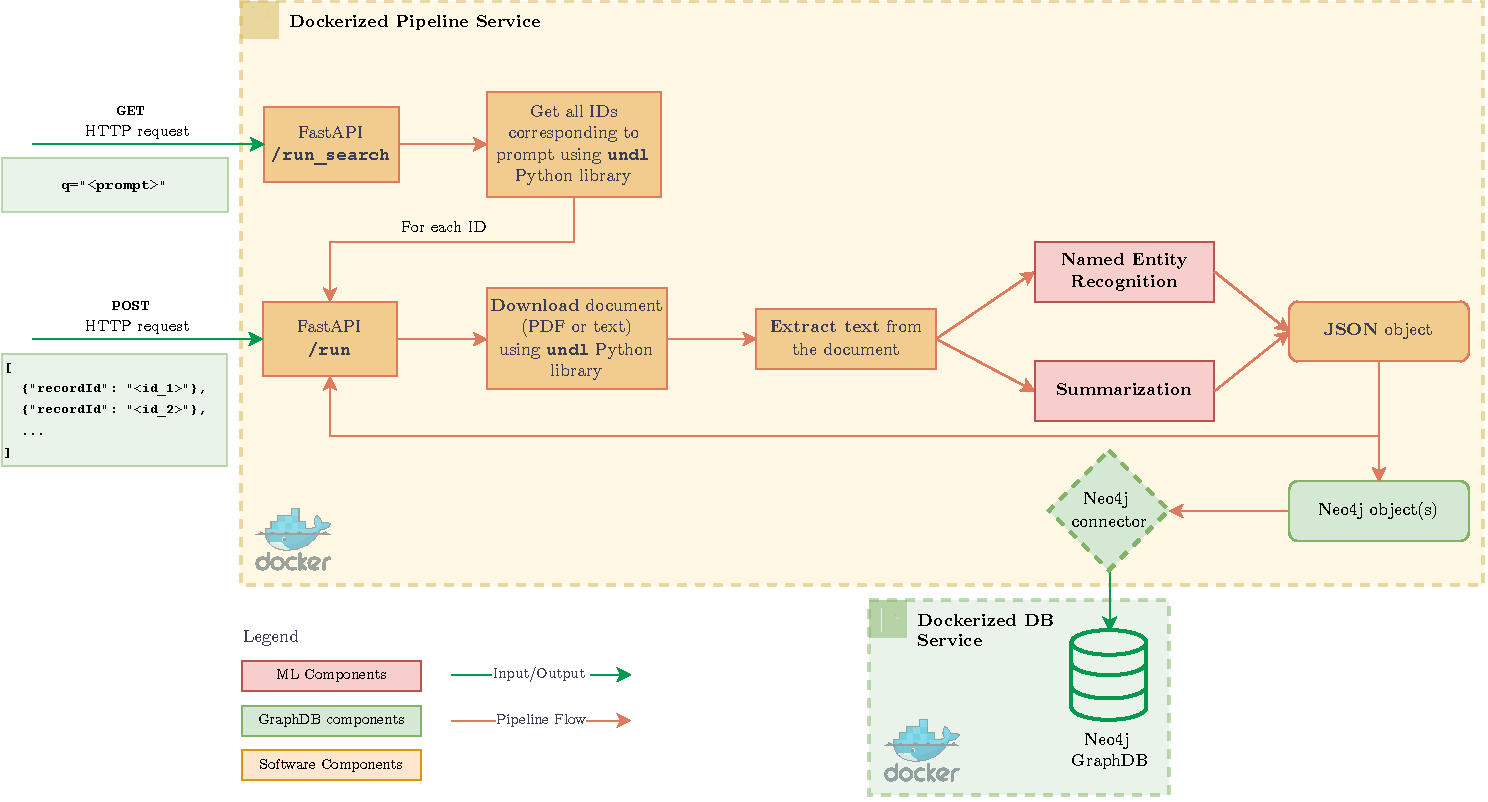
\includegraphics[width=\textwidth]{res/ml-pipeline.pdf}
    \caption{\texttt{un-semun-frontend} library: a dockerized machine learning pipeline for NER \& summarization}
    % change caption position to the bottom

    \label{fig:frontend-screenshot}
\end{figure}



\subsection{\texttt{un-semun-api}: An API for \texttt{un-semun-frontend} using FastAPI} \label{ssec:un-semun-api-an-api-for-un-semun-frontend-using-fastapi}
\subsubsection*{Tech stack of \texttt{un-semun-api}} \label{sssec:tech-stack-of-un-semun-api}

\subsection{\texttt{undl}: A Python library to wrap to the UN Digital Library API} \label{ssec:undl-a-python-library-to-wrap-to-the-un-digital-library-api}

\subsubsection*{Tech stack of \texttt{undl}} \label{sssec:tech-stack-of-undl}

For the \texttt{undl} library, I used Python 3.10 with packages, with \texttt{requests} for the HTTP requests, \texttt{pandas} for the data manipulation, and \texttt{pydantic} for the data validation.


\todo[inline]{Intermediary between frontend and Neo4j}
\todo[inline]{Proxying the UNDL API using \texttt{undl} library}

% UNBIST
\subsection{\texttt{un-unbis-thesaurus-scraper}: the UNBIS Thesaurus scraper} \label{ssec:un-unbis-thesaurus-scraper-the-unbis-thesaurus-scraper}

\subsubsection*{Tech stack of \texttt{un-unbis-thesaurus-scraper}} \label{sssec:tech-stack-of-un-unbis-thesaurus-scraper}


% unml
\subsection{\texttt{unml}: The machine learning pipeline} \label{ssec:unml-the-machine-learning-pipeline}

\subsubsection*{Tech stack of \texttt{un-ml-pipeline}} \label{sssec:tech-stack-of-un-ml-pipeline}

\subsubsection{Parts} \label{sssec:parts}

\todo[inline]{Parts}

\subsubsection{Models} \label{sssec:models}
\todo[inline]{Models}

\subsubsection{API} \label{sssec:api}
\todo[inline]{API}
\todo[inline]{Connection to Neo4j}


\begin{figure}[!htb]
    \centering

    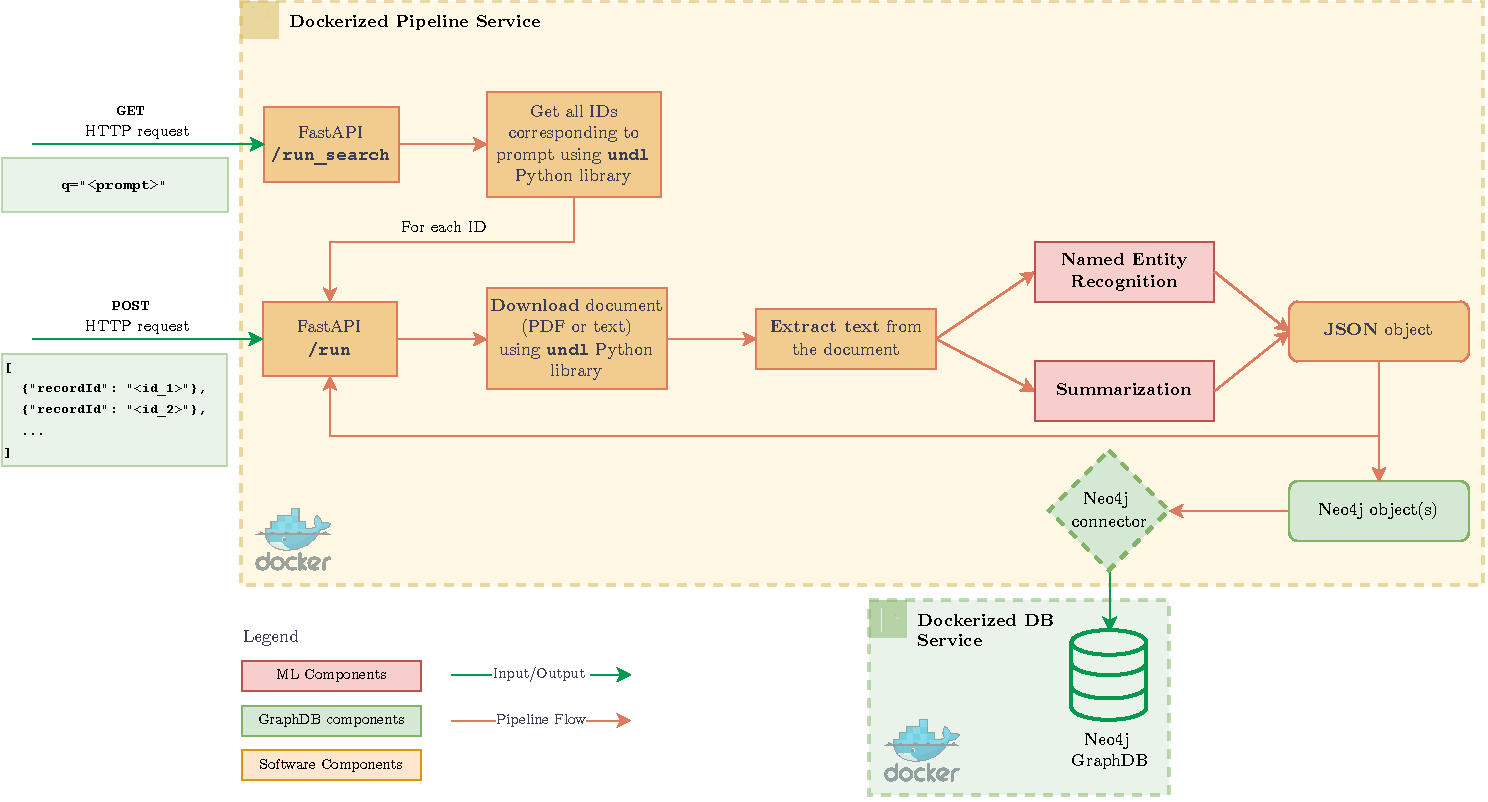
\includegraphics[width=\textwidth]{res/ml-pipeline.pdf}
    \caption{\texttt{unml} library: a dockerized machine learning pipeline for NER \& summarization}
    % change caption position to the bottom

    \label{fig:ml-pipeline}
\end{figure}



\subsection{Neo4j graph database} \label{ssec:neo4j-graph-database}

\subsubsection{Types of nodes} \label{sssec:types-of-nodes}
\todo[inline]{Types of nodes}

\subsubsection{Types of relationships} \label{sssec:types-of-relationships}
\todo[inline]{Types of relationships}


\subsection{\texttt{un-semun-misc}} \label{ssec:un-semun-misc}




\subsection{General tech stack notes} \label{ssec:general-tech-stack-notes}

For all the Python components, the dependencies are managed using \href{https://github.com/python-poetry/poetry}{\texttt{poetry}}. They are also all dockerized, and the whole stack is orchestrated using \href{https://docs.docker.com/compose/}{\texttt{docker-compose}}.

\section{Limitations} \label{sec:limitations}


The right of Figure \ref{fig:architecture} shows a simplified schema of the current UN Digital Library infrastructure.


\section{Discussion \& future work} \label{sec:discussion-future-work}

\section*{Conclusion} \label{sec:conclusion}

\end{document}